\section{模型检验与灵敏度分析}

\subsection{结果的可复现性与核数稳定性}\label{sec:repro}

论文和附录中的每一个 Makespan、搬运量和命中率，都来自终版复评：对每个（问题，用例，核数）选出的最优方案，把方案文件重新交给官方评估程序，在固定配置下再评一遍，并要求复评值与选优时记录的值逐位一致。终版复评共 1{,}400 个主结果（问题一 2--5 核、问题二 1--5 核、问题三 1--5 核各 100 个用例）和 500 组问题三同方案配对，全部通过，不一致数为 0。每个方案文件都记录了 SHA-256 哈希，附录中的数字与方案文件、评估输出之间可以逐项核对。

评估过程还跨越了两种运行环境：扫描、成组合并和局部搜索的大部分评估在云服务器（Python 3.10）上完成，终版复评在本机（Python 3.12）上进行，两者记录的 Makespan 逐位一致。这也验证了第 3 节的核内调度确定性假设，逐用例选优的比较是有意义的。

题目要求算法在 2--5 核范围内都能稳定生成高质量结果。经过算法~\ref{alg:select} 的核数补齐，问题一、二、三的全部 100 个用例都满足
\begin{equation}
  M_{k+1}\le M_k,\qquad k=2,3,4\ \ (\text{问题三为 }k=1,\dots,4),
  \label{eq:monotone}
\end{equation}
即多给一个核心，结果不会变差。补齐过程中，问题一、二、三分别评估了 \V{mono_p1}、\V{mono_p2}、\V{mono_p3} 个补空核方案（共 \V{mono_total} 个），经官方评估，其中 \V{mono_identical} 个的 Makespan 与原少核方案相同，没有一例因补空核而改变。

平均并行效率随核数下降（问题一从 2 核的 \V{p1_k2_eff_mean} 降到 5 核的 \V{p1_k5_eff_mean}），这是固定同步延迟和 DDR 共享带宽共同作用的结果，与第~\ref{sec:refs} 节可达参考的变化趋势一致：可达参考的 5 核平均加速比也只有 \V{p1_k5_ref_speedup_mean}（场景 A）和 \V{p2_k5_ref_speedup_mean}（场景 B）。计算图规模对达成率的影响不是简单的越大越好：4 核时达成率与 $\lg$(总计算周期) 的相关系数，问题一只有 \V{p1_k4_size_corr}，问题二为 \V{p2_k4_size_corr}。规模影响的是稳定性（图~\ref{fig:size}）：总计算量低于 $10^5$ 周期的 \V{p1_k4_small_n} 个小图，问题二达成率的标准差为 \V{p2_k4_small_achieve_sd}，$10^6$ 周期以上的大图只有 \V{p2_k4_large_achieve_sd}。小图的结果更依赖具体的依赖链形状，核数补齐也主要在小图上起作用。

\begin{figure}[H]
  \centering
  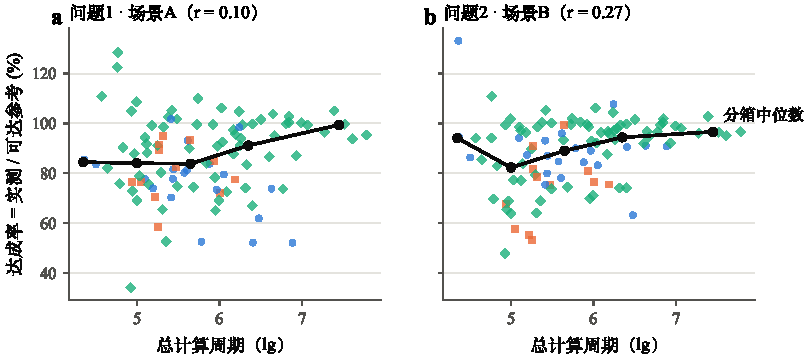
\includegraphics[width=\textwidth]{size_threshold}
  \caption{达成率与规模（4 核）。横轴为总计算周期（对数），折线为分箱中位数}
  \label{fig:size}
\end{figure}

\subsection{各求解环节的贡献}\label{sec:neg-record}

为了检验求解流程中每一步是否必要，我们按来源把候选逐步加入候选池，重新计算三个问题的平均加速比（表~\ref{tab:ladder}）。从朴素基线到三种构造算法逐用例选优，提升最大；成组合并在问题一中把 5 核平均加速比从 \V{ladder_p1_k5_sweep} 提到 \V{ladder_p1_k5_coarsen}，在问题二、三中增量较小；局部搜索、交叉复评和核数补齐每一步的平均增量都不大，但各自在一部分用例上是唯一的改进来源，所以都保留在最终流程中。

\begin{table}[H]
\centering
\caption{按来源逐步加入候选池后的平均加速比（累计；问题三为只读 Cache 配置相对官方单核基准）}
\label{tab:ladder}
\renewcommand\arraystretch{1.15}
\begin{tabular}{lcccccc}
\toprule
\multirow{2}{*}{候选来源} & \multicolumn{2}{c}{问题一} & \multicolumn{2}{c}{问题二} & \multicolumn{2}{c}{问题三} \\
\cmidrule(lr){2-3}\cmidrule(lr){4-5}\cmidrule(lr){6-7}
 & 4 核 & 5 核 & 4 核 & 5 核 & 4 核 & 5 核 \\
\midrule
朴素基线（分量装箱，$\alpha=0.25$） & \V{ladder_p1_k4_naive} & \V{ladder_p1_k5_naive} & \V{ladder_p2_k4_naive} & \V{ladder_p2_k5_naive} & \V{ladder_p3_k4_naive} & \V{ladder_p3_k5_naive} \\
三种构造算法逐用例选优 & \V{ladder_p1_k4_sweep} & \V{ladder_p1_k5_sweep} & \V{ladder_p2_k4_sweep} & \V{ladder_p2_k5_sweep} & \V{ladder_p3_k4_sweep} & \V{ladder_p3_k5_sweep} \\
\quad + 成组合并 & \V{ladder_p1_k4_coarsen} & \V{ladder_p1_k5_coarsen} & \V{ladder_p2_k4_coarsen} & \V{ladder_p2_k5_coarsen} & \V{ladder_p3_k4_coarsen} & \V{ladder_p3_k5_coarsen} \\
\quad + 局部搜索 & \V{ladder_p1_k4_localsearch} & \V{ladder_p1_k5_localsearch} & \V{ladder_p2_k4_localsearch} & \V{ladder_p2_k5_localsearch} & \V{ladder_p3_k4_localsearch} & \V{ladder_p3_k5_localsearch} \\
\quad + 交叉复评（仅问题二、三） & \V{ladder_p1_k4_crosseval} & \V{ladder_p1_k5_crosseval} & \V{ladder_p2_k4_crosseval} & \V{ladder_p2_k5_crosseval} & \V{ladder_p3_k4_crosseval} & \V{ladder_p3_k5_crosseval} \\
\quad + 核数补齐（最终） & \V{ladder_p1_k4_monotone} & \V{ladder_p1_k5_monotone} & \V{ladder_p2_k4_monotone} & \V{ladder_p2_k5_monotone} & \V{ladder_p3_k4_monotone} & \V{ladder_p3_k5_monotone} \\
\bottomrule
\end{tabular}
\end{table}

第~\ref{sec:neg} 节与第~\ref{sec:p3-solve} 节提到的未采用路线，都用当前代码重新运行过，结果文件保存在附件中。错开读取后处理在并发缺失占比最高的 \V{stagger_n} 个用例上（4 核，问题三），与不做错开相比：\V{stagger_better} 例改进（最多 \V{stagger_best_pct}），\V{stagger_same} 例不变，\V{stagger_worse} 例变差（最多变差 \V{stagger_worst_pct}）。这一方向在当前形式下不可用。

\subsection{参数灵敏度}

表~\ref{tab:param} 给出各构造算法在固定参数下的 4 核平均加速比（只列覆盖全部 100 个用例的参数值）。分量装箱的 $\alpha$ 越大越差，$\alpha\le 0.25$ 时分量不被切开，结果相同，说明对多分量图把整个分量放在一起几乎总是对的。层带划分的最优方向在两个场景下相反：问题一中 $W=16$（粗切）最好，问题二中 $W=4096$（细切）最好，这正是第~\ref{sec:p1-model} 节和第~\ref{sec:p2-model} 节的模型所预测的：场景 A 中路径上的子图边界是代价，场景 B 中只有换核才是。任何固定参数的平均值都明显低于逐用例选优（4 核问题一 \V{p1_k4_portfolio_mean}、问题二 \V{p2_k4_portfolio_mean}），而同一算法内逐用例调参的收益很小（例如分量装箱从固定 $\alpha=0.25$ 的 \V{sens_p1_lpt_0p25} 到逐用例最优的 \V{p1_k4_lpt_mean}）。对这批用例，选对构造算法比在同一算法内调参重要得多。

\begin{table}[H]
\centering
\caption{构造算法在固定参数下的 4 核平均加速比}
\label{tab:param}
\renewcommand\arraystretch{1.15}
\begin{tabular}{llcc}
\toprule
算法 & 参数取值 & 问题一 & 问题二 \\
\midrule
\multirow{7}{*}{分量装箱 $\alpha$}
 & 0.1 & \V{sens_p1_lpt_0p1} & \V{sens_p2_lpt_0p1} \\
 & 0.25 & \V{sens_p1_lpt_0p25} & \V{sens_p2_lpt_0p25} \\
 & 0.5 & \V{sens_p1_lpt_0p5} & \V{sens_p2_lpt_0p5} \\
 & 1 & \V{sens_p1_lpt_1} & \V{sens_p2_lpt_1} \\
 & 2 & \V{sens_p1_lpt_2} & \V{sens_p2_lpt_2} \\
 & 4 & \V{sens_p1_lpt_4} & \V{sens_p2_lpt_4} \\
 & 8 & \V{sens_p1_lpt_8} & \V{sens_p2_lpt_8} \\
\midrule
\multirow{3}{*}{层带划分 $W$}
 & 16 & \V{sens_p1_band_16} & \V{sens_p2_band_16} \\
 & 256 & \V{sens_p1_band_256} & \V{sens_p2_band_256} \\
 & 4096 & \V{sens_p1_band_4096} & \V{sens_p2_band_4096} \\
\midrule
\multirow{3}{*}{相位构造 $\lambda$}
 & 2000 & \V{sens_p1_phase_2000} & \V{sens_p2_phase_2000} \\
 & $10^4$ & \V{sens_p1_phase_10000} & \V{sens_p2_phase_10000} \\
 & $5\times10^4$ & \V{sens_p1_phase_50000} & \V{sens_p2_phase_50000} \\
\bottomrule
\end{tabular}
\end{table}

\subsection{硬件参数扰动下的鲁棒性}

官方配置是固定的，但实际硬件的带宽和同步开销会有波动。我们检验本文方案的优势是否依赖于某个具体参数：从三类中各取 10 个用例（按编号等间隔抽取），在 4 核下把 DDR 带宽改为 48、72 bytes/cycle（$\pm20\%$），或把同步相关的等待与延迟同时乘以 0.8、1.2，分别评估本文的最终方案和朴素方案（分量装箱，$\alpha=0.25$）。注意本文方案是在官方配置下选出的，扰动后没有重新优化。结果见表~\ref{tab:robust}。

\begin{table}[H]
\centering
\caption{参数扰动下本文方案相对朴素方案的 Makespan 比（几何平均，大于 1 表示本文更快；4 核，\V{rob_p1_official_n} 个用例）}
\label{tab:robust}
\renewcommand\arraystretch{1.15}
\begin{tabular}{lcccc}
\toprule
\multirow{2}{*}{配置} & \multicolumn{2}{c}{问题一} & \multicolumn{2}{c}{问题二} \\
\cmidrule(lr){2-3}\cmidrule(lr){4-5}
 & 朴素 / 本文 & 本文方案 Makespan 变化 & 朴素 / 本文 & 本文方案 Makespan 变化 \\
\midrule
官方配置 & \V{rob_p1_official_adv} & 1.00 & \V{rob_p2_official_adv} & 1.00 \\
DDR 带宽 48 & \V{rob_p1_bw48_adv} & \V{rob_p1_bw48_ms_ratio} & \V{rob_p2_bw48_adv} & \V{rob_p2_bw48_ms_ratio} \\
DDR 带宽 72 & \V{rob_p1_bw72_adv} & \V{rob_p1_bw72_ms_ratio} & \V{rob_p2_bw72_adv} & \V{rob_p2_bw72_ms_ratio} \\
同步开销 $\times 0.8$ & \V{rob_p1_sync08_adv} & \V{rob_p1_sync08_ms_ratio} & \V{rob_p2_sync08_adv} & \V{rob_p2_sync08_ms_ratio} \\
同步开销 $\times 1.2$ & \V{rob_p1_sync12_adv} & \V{rob_p1_sync12_ms_ratio} & \V{rob_p2_sync12_adv} & \V{rob_p2_sync12_ms_ratio} \\
\bottomrule
\end{tabular}
\end{table}

四种扰动下，本文方案相对朴素方案的优势基本不变：问题一保持在 \V{rob_p1_sync12_adv}--\V{rob_p1_sync08_adv} 倍、问题二保持在 \V{rob_p2_bw48_adv}--\V{rob_p2_sync08_adv} 倍。逐用例看，只有问题二带宽降为 48 时有 \V{rob_p2_bw48_nworse} 个用例本文方案略慢于朴素方案（比值 \V{rob_p2_bw48_minadv}），其余配置下没有一例反超。本文方案自身的 Makespan 随带宽下降而增加、随同步开销增加而增加，方向与模型一致，幅度都在 3\% 以内。这说明方案的优势来自结构性的切分方式，而不是对某组参数的过拟合。

\subsection{运行时间}

三种构造算法本身都很快。在本机（负载较高时）单进程测量，4 核方案的生成时间中位数为：分量装箱 \V{time_lpt_median} 秒、层带划分 \V{time_band_median} 秒、相位构造 \V{time_phase_median} 秒；最大的用例 \V{time_bigcase}（\V{time_bigcase_ops} 个操作）上最慢的一次也只需 \V{time_all_max} 秒。耗时主要在官方评估程序上。题目要求单个用例以 5--10 分钟内给出结果为佳，我们在最大用例上实测了附件程序的快速模式（9 个构造候选加 21 个成组合并变体，共 30 次官方评估）：CPU 时间合计约 \V{figx_fast_big_cpu_min} 分钟，8 进程并行时墙钟时间约 1 分钟。快速模式的求解质量见第 5.4.2、5.7.2 与 5.10.2 节，仅用 9 个构造候选时，5 核平均加速比已达最终结果的 90\%--96\%。由局部搜索的记录推算，单次评估的中位数为 \V{eval_secs_median} 秒，最大的用例上约 \V{eval_secs_max} 秒。

附件程序只依赖 Python 3.10 及以上版本的标准库和赛题官方材料包，提供两种运行方式。求解入口 \texttt{solve.py} 对给定计算图与核数运行三种构造算法（各 3 组代表参数）和成组合并，由官方评估程序选出最优方案，单个用例一般在数分钟内完成；复现入口 \texttt{reproduce.py} 读取本文的 1{,}400 个最终方案文件并调用官方评估程序，逐项复现附录中的数字。三种构造算法分别实现在 \texttt{nmcs/algos.py}、\texttt{algos2.py}、\texttt{algos4.py} 中，参数扫描、后处理与统计作图的完整实验代码在 \texttt{research\_code/} 目录下。
